\documentclass[13pt, a4paper,headinclude, 
footinclude, 
plainfootsepline]{scrreprt} % Defines the font size and the paper format

\usepackage[english]{babel}
\usepackage[utf8]{inputenc}
\usepackage{textcomp}
\usepackage{amsmath, amssymb, amsfonts} % Standard AMS packages
\usepackage{amsthm}           % For theorem environments
\usepackage{geometry}         % Customize page geometry
\usepackage{setspace}         % To set line spacing
\usepackage{graphicx}
\usepackage[automark,headsepline,footsepline]{scrpage2}
\usepackage{pdfpages}
\usepackage{color}
\usepackage{listings}
\usepackage{float}
\usepackage{pgfplots,pgfplotstable}
\usepackage{caption}
\usepackage{setspace}

%--------------------------------------------------------------------
%--- Configure Listing Design
%--------------------------------------------------------------------
\definecolor{pblue}{rgb}{0.13,0.13,1}
\definecolor{pgreen}{rgb}{0,0.5,0}
\definecolor{pred}{rgb}{0.9,0,0}
\definecolor{pgrey}{rgb}{0.46,0.45,0.48}

\lstdefinestyle{lstStyle}{
	language=java,
	numbers=left,
	stepnumber=1,
	numbersep=10pt,
	tabsize=4,
	showspaces=false,
	showstringspaces=false
}

\lstset{
	basicstyle=\tiny,
	style=lstStyle,
	frame=tb,
	language=Java,
	showspaces=false,
	showtabs=false,
	breaklines=true,
	columns=fullflexible,
	showstringspaces=false,
	breakatwhitespace=true,
	basicstyle=\ttfamily,
	tabsize=3
}
%--------------------------------------------------------------------
%--- Title, author, date
%--------------------------------------------------------------------

\newcommand{\theuniversity}{Brunel University London}
\newcommand{\thecollege}{College of Engineering, Design and Physical Sciences}
\newcommand{\thedepartment}{Department of Engineering and Design}
\newcommand{\thecoursetitle}{Assignment \\ Workshop EE5614}
\newcommand{\thestudent}{Tobias \textsc{Schwarz}}
\newcommand{\thestudentid}{1744864}
\newcommand{\thestudenttwo}{Stephan \textsc{Dittmann}}
\newcommand{\thestudentidtwo}{1744874}
\newcommand{\thestudentthree}{Roland \textsc{Flat}}
\newcommand{\thestudentidthree}{1744872}
\newcommand{\thesupervisor}{Satikidis Dionysis}
\newcommand{\theyear}{2018}
\newcommand{\thetitle}{Embedded Systems}
\newcommand{\code}[1]{\texttt{#1}}


%--------------------------------------------------------------------
%--- Global page geometry and layout
%--------------------------------------------------------------------

% Define the page margins
\geometry{
	left=40mm,
	right=25mm,
	bindingoffset=0mm, 
	top=25mm,
	bottom=25mm,
	headsep=15mm
}
\setlength\parindent{0pt}
\addtokomafont{disposition}{\rmfamily}
\pagestyle{scrheadings}
\renewcommand*{\chapterheadstartvskip}{\vspace*{-0.5cm}}
\renewcommand*{\chapterheadendvskip}{\vspace{7.5mm}}
\renewcommand{\chapterpagestyle}{scrheadings}
% Kopf- und Fußzeile auch auf Kapitelanfangsseiten
\clearscrheadfoot
% Schriftform der Kopfzeile
\renewcommand{\headfont}{\normalfont}
% Kopfzeile
\ihead{Project Control and Management}
\chead{}
\ohead{
\includegraphics[scale=0.15]{BasePictures/Brunel_University_Logo.png}}
%Fußzeile
\ifoot[Tobias Schwarz]{Tobias Schwarz, Stephan Dittmann, Roland Flat}
\ofoot[\pagemark]{\pagemark}
\setheadsepline{.5pt}
\setfootsepline{.5pt}
%---------------------------------------------------------------------
%--- Theorem environments
%---------------------------------------------------------------------

% Theorem counter is subordinate to chapter; all theorem-like
% environments are using the same counter
\theoremstyle{plain}
\newtheorem{theorem}{Theorem}[chapter]          
\newtheorem{lemma}[theorem]{Lemma}
\newtheorem{proposition}[theorem]{Proposition}
\newtheorem{corollary}[theorem]{Corollary}

\theoremstyle{definition}
\newtheorem{definition}[theorem]{Definition}
\newtheorem{remark}[theorem]{Remark}

%---------------------------------------------------------------------
%--- Bibliography
%---------------------------------------------------------------------

\usepackage[style=numeric, minnames=3,
            doi=false, url=false, isbn=false,
            firstinits=true,
            sortcites=true,
            backend=bibtex]{biblatex}

\addbibresource{bibliography.bib}

%---------------------------------------------------------------------
%--- Document begins here
%---------------------------------------------------------------------

\begin{document}
	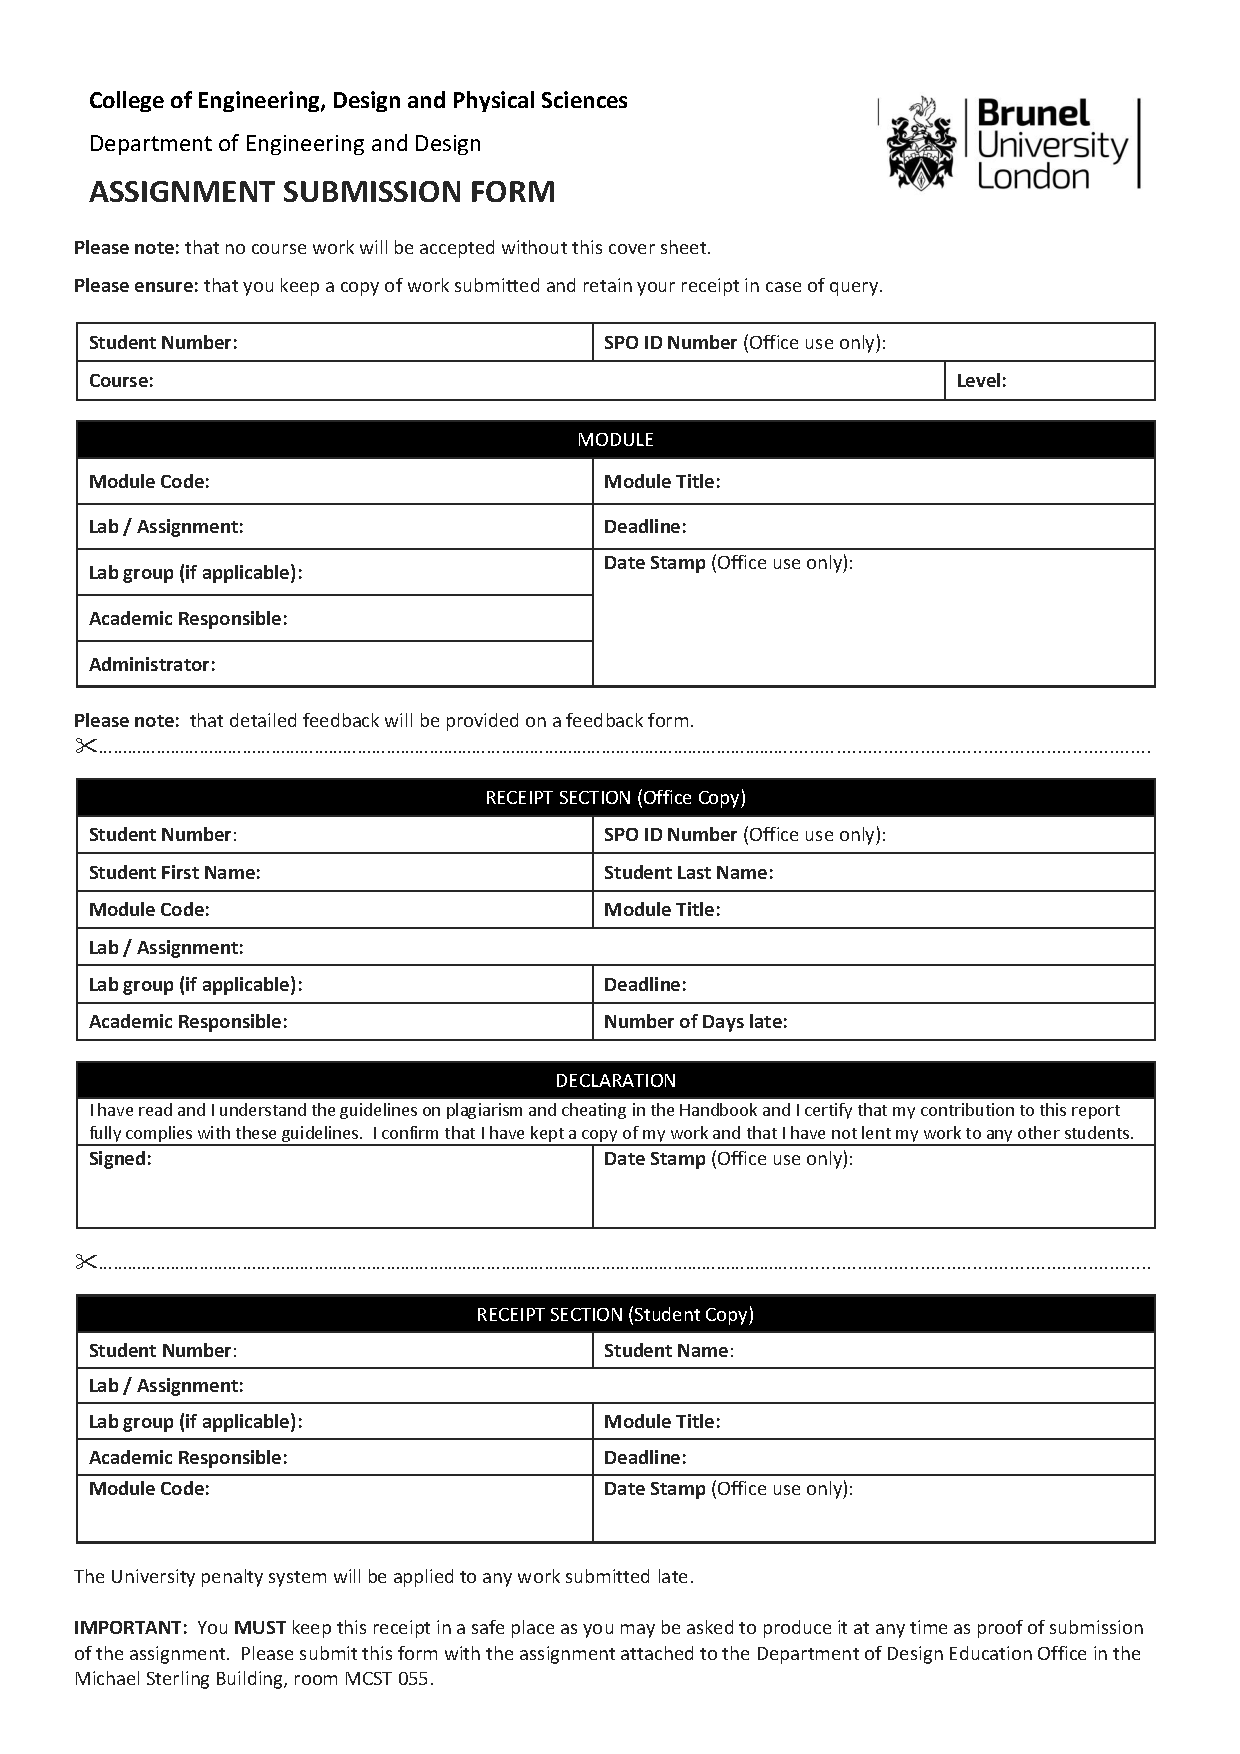
\includepdf{BasePictures/SubmissionForm.pdf}
	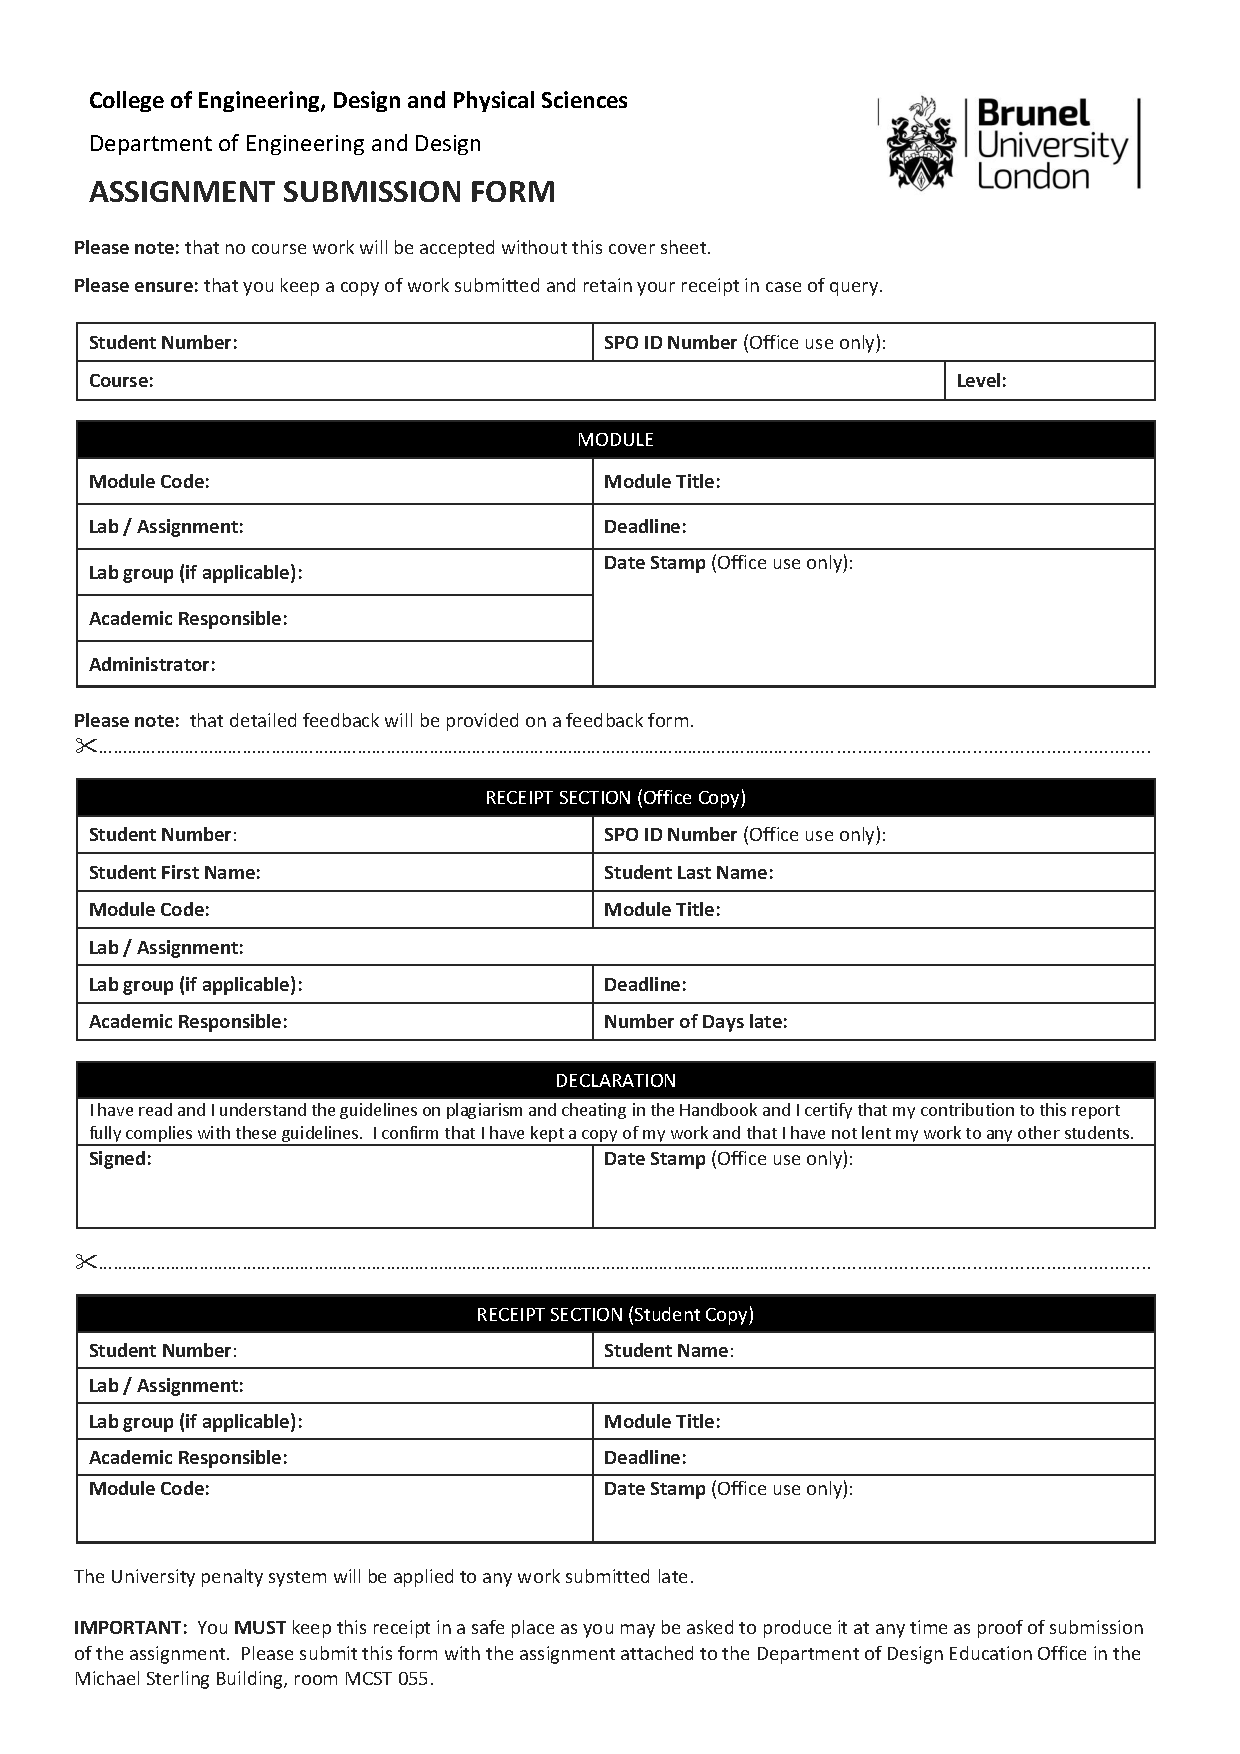
\includepdf{BasePictures/SubmissionForm.pdf}
	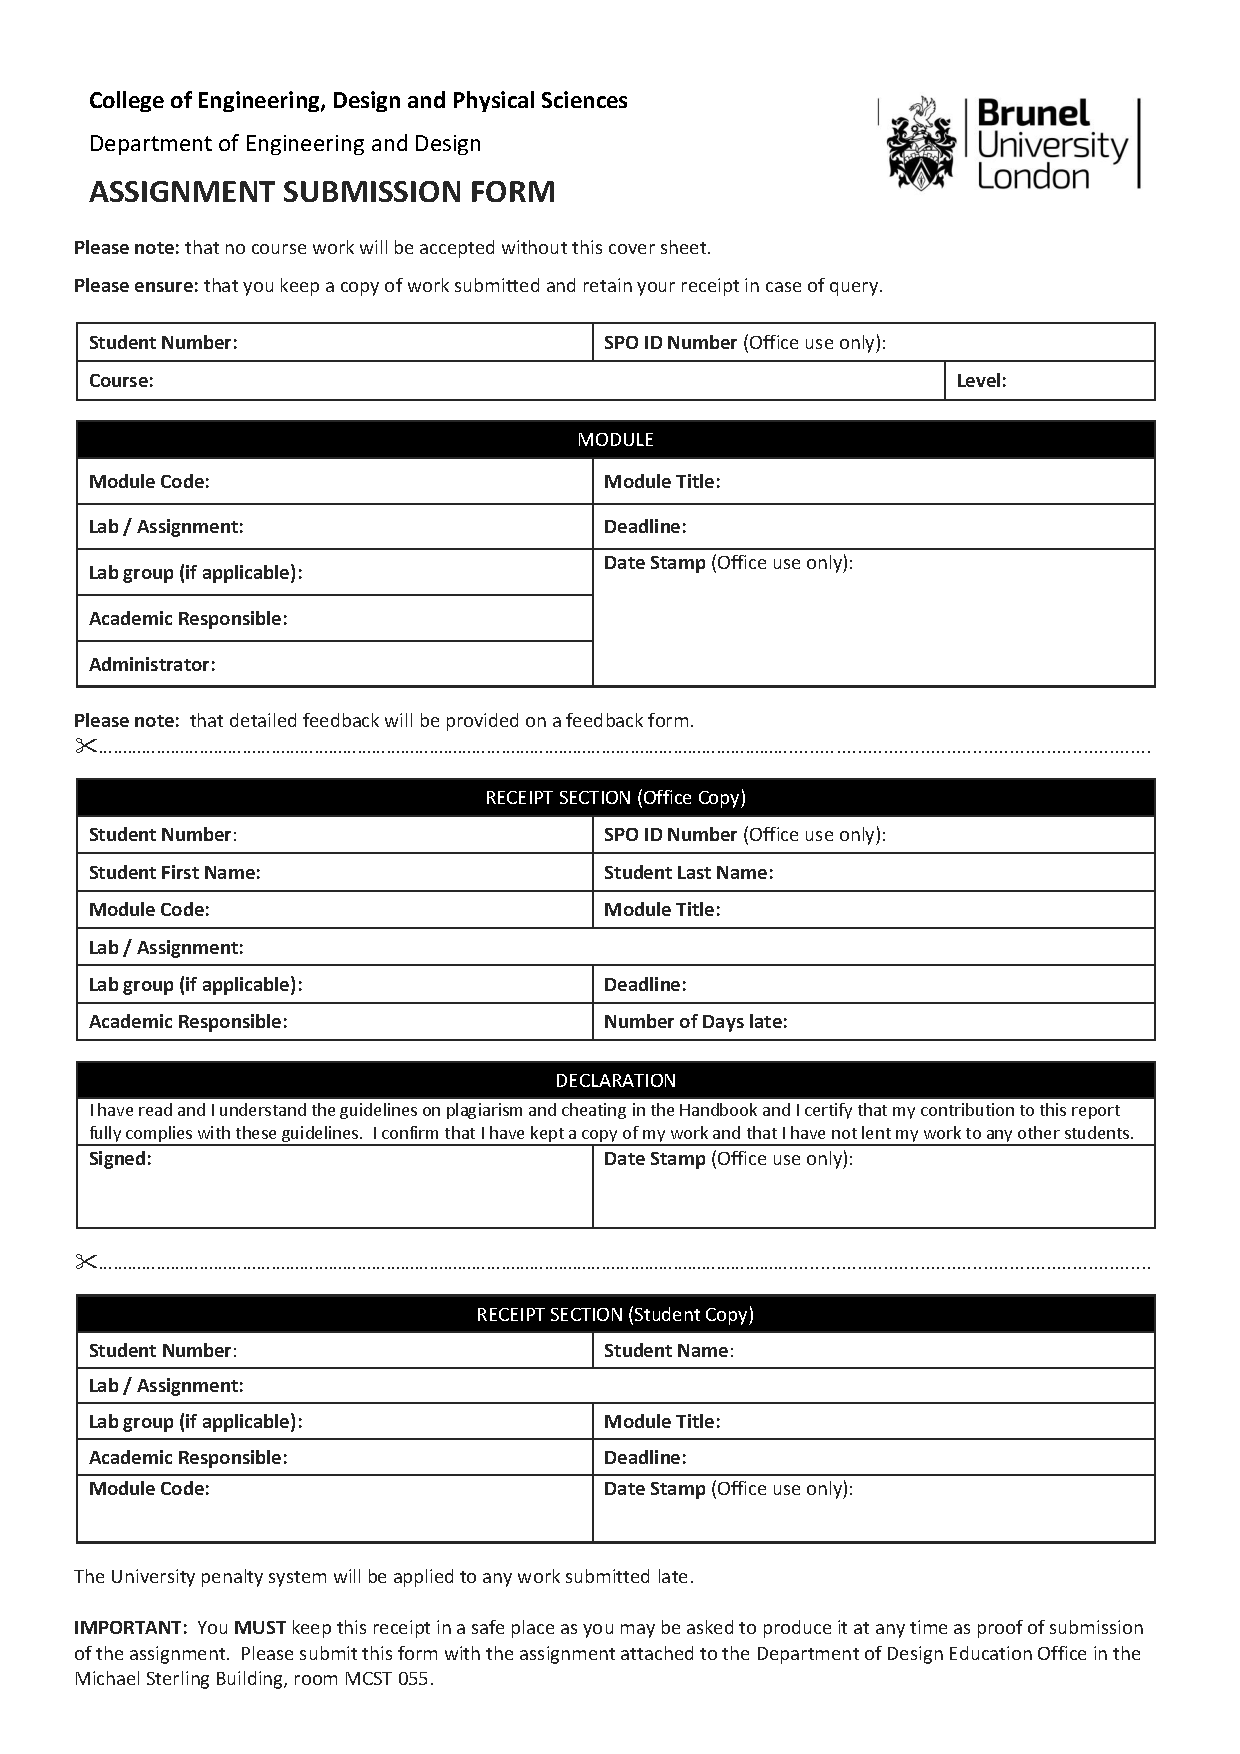
\includepdf{BasePictures/SubmissionForm.pdf}
\onehalfspacing

%---------------------------------------------------------------------
%--- Title page
%---------------------------------------------------------------------

\begin{titlepage}
	\center
	
	% Name of university, college, department and degree
	\textsc{\LARGE \theuniversity} \\[1.5cm] 
	\textsc{\large 
		\thecollege \\
		\thedepartment} \\[1.5cm]
	\textsc{\Large \thecoursetitle} \\[3.0cm]
	
	% Project title
	\rule{\linewidth}{0.5mm} \\[0.5cm]
	{ \huge\textbf{ \thetitle } } \\
	\rule{\linewidth}{0.5mm} \\[5cm]
	
	% Student name, student number and supervisor
	\begin{minipage}{0.4\textwidth}
		\begin{flushleft} \large
			\thestudent \\
			Student Number: \thestudentid \\
			\thestudenttwo \\
			Student Number: \thestudentidtwo \\
			\thestudentthree \\
			Student Number: \thestudentidthree
		\end{flushleft}
	\end{minipage}
	~
	\begin{minipage}{0.4\textwidth}
		\begin{flushright} \large
			\emph{Supervisor:} \\
			\thesupervisor
		\end{flushright}
	\end{minipage}\\[1cm]
	
	% Year
	{\large Year of Submission: \theyear} \\[3cm] 
	
	\vfill % Fill the rest of the page with whitespace
\end{titlepage}
\newpage

%---------------------------------------------------------------------
%--- Front matter
%---------------------------------------------------------------------

\pagenumbering{roman}

\tableofcontents
\listoffigures
\newpage

%---------------------------------------------------------------------
%--- Main part of thesis
%---------------------------------------------------------------------

\pagenumbering{arabic}

\input{Chapters/Kapitel.tex}
\input{Chapters/Kapitel2.tex}
\input{Chapters/Kapitel3.tex}
\input{Chapters/Kapitel4.tex}
\input{Chapters/Kapitel5.tex}

%---------------------------------------------------------------------
%--- Bibliography and appendices
%---------------------------------------------------------------------



		
\end{document}
